\documentclass[12pt,letterpaper]{exam}
\usepackage[lmargin=1in,rmargin=1in,tmargin=1in,bmargin=1in]{geometry}
\usepackage{../style/exams}

% -------------------
% Course & Exam Information
% -------------------
\newcommand{\course}{MAT 101: Exam 2}
\newcommand{\term}{Fall -- 2022}
\newcommand{\examdate}{10/26/2022}
\newcommand{\timelimit}{60 Minutes}

\setbool{hideans}{true} % Student: True; Instructor: False

% -------------------
% Content
% -------------------
\begin{document}

\examtitle
\instructions{Write your name on the appropriate line on the exam cover sheet. This exam contains \numpages\ pages (including this cover page) and \numquestions\ questions. Check that you have every page of the exam. Answer the questions in the spaces provided on the question sheets. Be sure to answer every part of each question and show all your work.} 
\scores
%\bottomline
\newpage

% ---------
% Questions
% ---------
\begin{questions}

% Question 1
\question[10] Suppose $f(x)$ is the relation given below.
	\[
	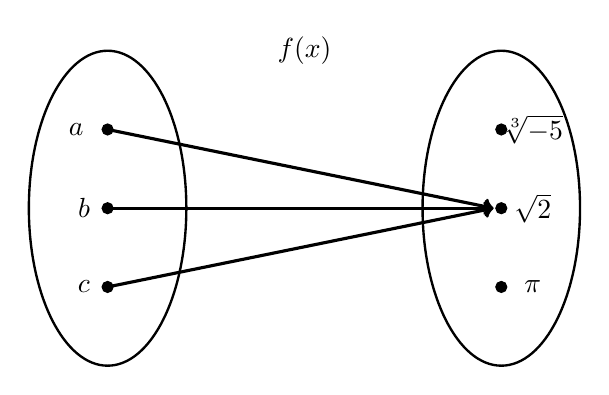
\begin{tikzpicture}
	\node at (2.5,2) {$f(x)$};
	% Ellipses
	\draw[line width=0.03cm] (0,0) circle (1 and 2);
	\draw[line width=0.03cm] (5,0) circle (1 and 2);
	
	% Nodes
	\draw[fill=black] (0,1) circle (0.07);
	\draw[fill=black] (0,0) circle (0.07);
	\draw[fill=black] (0,-1) circle (0.07);
	
	\draw[fill=black] (5,1) circle (0.07);
	\draw[fill=black] (5,0) circle (0.07);
	\draw[fill=black] (5,-1) circle (0.07);
	
	% Arrow
	\draw[line width=0.04cm,->] (0,1) -- (4.9,0);
	\draw[line width=0.04cm,->] (0,0) -- (4.9,0);
	\draw[line width=0.04cm,->] (0,-1) -- (4.9,0);
	
	% Labels
	\node at (-0.4,1) {$a$};
	\node at (-0.3,0) {$b$};
	\node at (-0.3,-1) {$c$};
	
	\node at (5.4,1) {$\sqrt[3]{-5}$};
	\node at (5.4,0) {$\sqrt{2}$};
	\node at (5.4,-1) {$\pi$};
	\end{tikzpicture}
	\]

\begin{enumerate}[(a)]
\item Is $f(x)$ a function? Explain.
\item What is the domain of $f(x)$?
\item What is the codomain of $f(x)$?
\item What is the range of $f(x)$?
\end{enumerate}



% Question 2
\newpage
\question[10] Is $f(x)= \dfrac{1 - x^3}{x^2 + 5}$ a function? Explain. 



% Question 3
\newpage
\question[10] Let $f(x, y)= (x - y)^2 - x + \dfrac{10}{y}$. Find $f(3, -2)$ and $f(4, 5)$. 



% Question 4
\newpage
\question[10] Let $f(x)= 4 - x^3$ and observe that $f(2)= -4$. 
	\begin{enumerate}[(a)]
	\item Is $(-1, 3)$ on the graph of $f(x)$? Explain. 
	\item Is $(2, -4)$ on the graph of $f(x)$? Explain. 
	\end{enumerate}



% Question 5
\newpage
\question[10]
Suppose $f(x)$ and $g(x)$ are the functions given below. 
        \begin{table}[!ht]
        \centering
        \begin{tabular}{| c || c | c | c | c | c | c | c |} \hline
	$x$ & $-3$ & $-2$ & $-1$ & $\phantom{-}0$ & $\phantom{-}1$ & $\phantom{-}2$ & $\phantom{-}3$ \\ \hline
	$f(x)$ & $\phantom{-}0$ & $\phantom{-}5$ & $\phantom{-}4$ & $-1$ & $-5$ & $-1$ & $-3$ \\ \hline
	$g(x)$ & $\phantom{-}1$ & $\phantom{-}2$ & $10$ & $\phantom{-}3$ & $\phantom{-}4$ & $-7$ & $\phantom{-}5$  \\ \hline
        \end{tabular}
        \end{table}

Compute the following: 
        \begin{enumerate}[(a)]
	\item $(f - g)(-1)$
	\item $(fg)(2)$
	\item $(-5g)(-2)$
	\item $(f \circ g)(0)$
	\item $(g \circ f)(0)$
        \end{enumerate} 



% Question 6
\newpage
\question[10] Let $f(x)$ be a function such that $f^{-1}(x)$ exists. A partial table of values for $f(x)$ is given below: \par
	\begin{table}[!ht]
	\centering
	\begin{tabular}{|r||c|c|c|c|c|} \hline 
	$x$ & $1$ & $2$ & $4$ & $8$ & $15$ \\ \hline
	$f(x)$ & $-2$ & $0$ & $6$ & $2$ & $10$ \\ \hline
	\end{tabular}
	\end{table}
Based on the table above (or your knowledge of functions and inverses), find the following:
	\begin{enumerate}[(a)]
	\item $f(2)$
	\item $f^{-1}(2)$
	\item $f^{-1}(f(2))$
	\item $f \big(f^{-1}(\pi) \big)$
	\item $f^{-1} \big( f(\sqrt{2}) \big)$
	\end{enumerate}



% Question 7
\newpage
\question[10] Let $f(x)= 5 - 6x$. Assume that $f^{-1}(x)$ exists and observe that $f(2)= -7$.
	\begin{enumerate}[(a)]
	\item What is $f^{-1}(-7)$? Explain. 
	\item Find $f^{-1}(17)$.
	\end{enumerate}



% Question 8
\newpage
\question[10] A graph of a relation $f(x)$ is shown below:
	\[
	\fbox{
	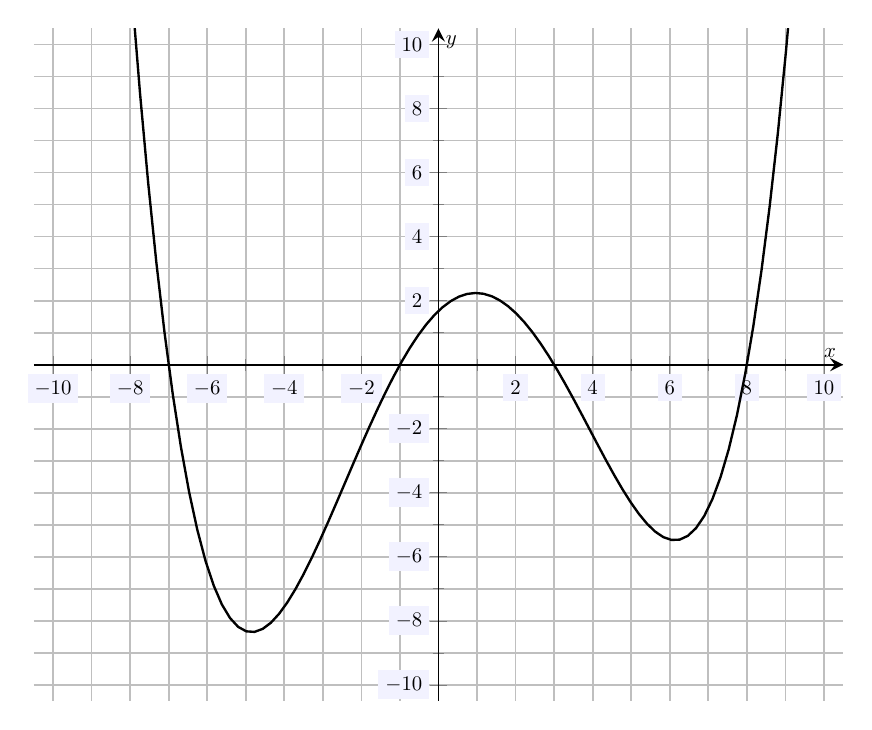
\begin{tikzpicture}[scale=1.5,every node/.style={scale=0.5}]
	\begin{axis}[
	grid=both,
	axis lines=middle,
	ticklabel style={fill=blue!5!white},
	xmin= -10.5, xmax=10.5,
	ymin= -10.5, ymax=10.5,
	xtick={-10,-8,-6,-4,-2,0,2,4,6,8,10},
	ytick={-10,-8,-6,-4,-2,0,2,4,6,8,10},
	minor tick = {-10,-9,...,10},
	xlabel=\(x\),ylabel=\(y\),
	]
	\addplot[line width= 0.02cm,samples=100,domain= -10.5:10.5] ({x},{1/100*(x+7)*(x+1)*(x-3)*(x-8)}); 
	\end{axis}
	\end{tikzpicture}
	}
	\] 
Using the graph above, answer the following:
	\begin{enumerate}[(a)]
	\item Is the relation $f(x)$ a function? Explain.
	\item Does the relation $f(x)$ have an inverse function? Explain. 
	\end{enumerate}



% Question 9
\newpage
\question[10] Let $f(x)= \dfrac{7 - x}{2}$ and $g(x)= 7 - 2x$. Show that $g(x)$ is the inverse of $f(x)$. 



% Question 10
\newpage
\question[10] Let $f(x)= 5x - 4$. Find $f^{-1}(x)$. 


\end{questions}
\end{document}